
\documentclass[8pt]{article}
%	options include 12pt or 11pt or 10pt
%	classes include article, report, book, letter, thesis

\usepackage[a4paper,bindingoffset=0.2in,%
            left=0.6in,right=0.6in,top=0.2in,bottom=0.4in,%
            footskip=.15in]{geometry}
            
\usepackage[T1]{fontenc}
\usepackage[polish]{babel}
\usepackage[utf8]{inputenc}
\usepackage{lmodern}
\selectlanguage{polish}
\usepackage{blindtext}
\usepackage{pgfplots}
\usepackage{graphicx}
\usepackage{color,colortbl}
\usepackage{hyperref}

\title{Aplikacje uniwersalne}
\author{Projekt / Semestr 6\\ Aleksander Kosma\\grupa 2 tester-programista}
\date{20 Marzec 2018}

\begin{document}
\maketitle 

\section*{Dokumentacja projektu}
\subsection*{ Opis projektu - Gym Progress}
Aplikacja ma pomóc w notowaniu progresu z siłowni. Można aplikacje wykorzystać wszędzie tam gdzie mamy kontakt z zapisem ćwiczeń w formie seria-powtórzenie. Dzięki zebranym danym aplikacja będzie mogła podać statystyki i metadane odnośnie naszych zmagań.\\
\\

Funkcjonalności aplikacji: \\
\textbf{Dodaj/Edytuj/Usuń trening} - w tej aktywności użytkownik odnotowuje ćwiczenia które wykonał na treningu. Z listy wybiera konkretne ćwiczenie, następnie ustala ilość serii i ciężar.\\

\textbf{Dodaj/Edytuj/Usuń ćwiczenie} - użytkownik może dodać nowe ćwiczenie jeśli nie ma go jeszcze na liście dostępnych.\\

\textbf{Wyświetl progres w formie statystyki} - Aplikacja sumuje ciężar z każdego treningu i zamieszcza dane w formie tabeli. Możliwe będą różne opcje wyświetlania danych.\\

\textbf{Wyświetl spis wszystkich treningów} - korzystający będzie mógł przeglądać dodane wcześniej treningi jak i je edytować lub usuwać.

\subsection*{ Opis funkcjonalności}
Menu aplikacji będzie składało się z 4 guzików i logo aplikacji. Korzystający będzie miał do wyboru dodanie treningu, spis treningów i spis dostępnych ćwiczeń. Ostatnia zakładka to wyświetlenie podsumowania treningów. W zakładce dodawania treningu będzie można określić datę treningu i jego krótki opis. Następnie należałoby wybrać ćwiczenia które wykonało się na treningu. Po kliknięciu dodawania ćwiczenia otworzy się kolejna zakładka do wyboru ćwiczenia i ustalenia ilości serii, powtórzeń i obciążenia. Po wykonaniu tych operacji można zapisać trening. W kolejnej zakładce można obejrzeć dodane treningi i je przeedytować jeśli jest potrzeba. Zakładka ćwiczeń pozwala nam na dodanie nowych ćwiczeń. Zakładka statystyk wyświetli nam podsumowanie każdego treningu z wyświetloną obok datą. Dzięki temu jasno widać progres w rozwoju. \\
.\\
\\
\\
\\
\\
\\
\\
\\
\\
\\
\\
\\
\\
\\
\\
\\
\\
\subsection*{ Przypadki użycia}
Tabela z przypadkami użycia: \\

\renewcommand{\arraystretch}{1}
\begin{tabular}{ | p{5.2cm} | p{5.2cm} | p{5.2cm} | }
  \hline
  \multicolumn{3}{|c|}{Przypadki użycia} \\\hline
  Nazwa & Opis & Inicjacja \\\hline
  Dodanie treningu & korzystający dodaje nowy trening wypełniając pola & Uruchomienie
  pierwszej zakładki w menu \\\hline
  Dodanie ćwiczenia & korzystający dodaje nowe ćwiczenie do już istniejących & Uruchomienie trzeciej zakładki w menu \\\hline
  Wyświetlenie dodanych treningów & Korzystający ma podgląd dodanych treningów & Uruchomienie drugiej zakładki w menu \\\hline
  Edycja treningu & Korzystający edytuje trening wraz z dodanymi do niego ćwiczeniami i opisem & Uruchomienie zakładki spisu treningów, następnie wybór treningu do edycji \\\hline
  Usunięcie treningu & Korzystający usuwa trening wraz z dodanymi do niego ćwiczeniami i opisem & Uruchomienie zakładki spisu treningów, następnie wybór treningu do usunięcia poprzez guzik \\\hline
  Wyświetlenie danych w formie statystyki & Korzystający ma podgląd do zsumowanej objętości z treningów w formie tabelki & Uruchomienie ostatniej zakładki w menu \\\hline
  Dodanie ćwiczenia w treningu & Korzystający ustala szczegóły danego ćwiczenia na treningu & Uruchomienie zakładki dodawania treningu następnie dodawania ćwiczenia do treningu \\\hline
  
  \hline
\end{tabular}
\subsection*{ Koncept wyglądu aplikacji i szczegóły}

Aplikacja będzie realizowana przy pomocy technologi Xamarin Forms. Docelowo aplikacja będzie działać na Windows jak i Android. Dane będą przechowywane w bazie danych SQL. Struktura projektu będzie w formie MVVM.\\
Poniżej znajduję się prawdopodobny wygląd menu aplikacji:\\
\begin{center}
 \makebox[\textwidth]{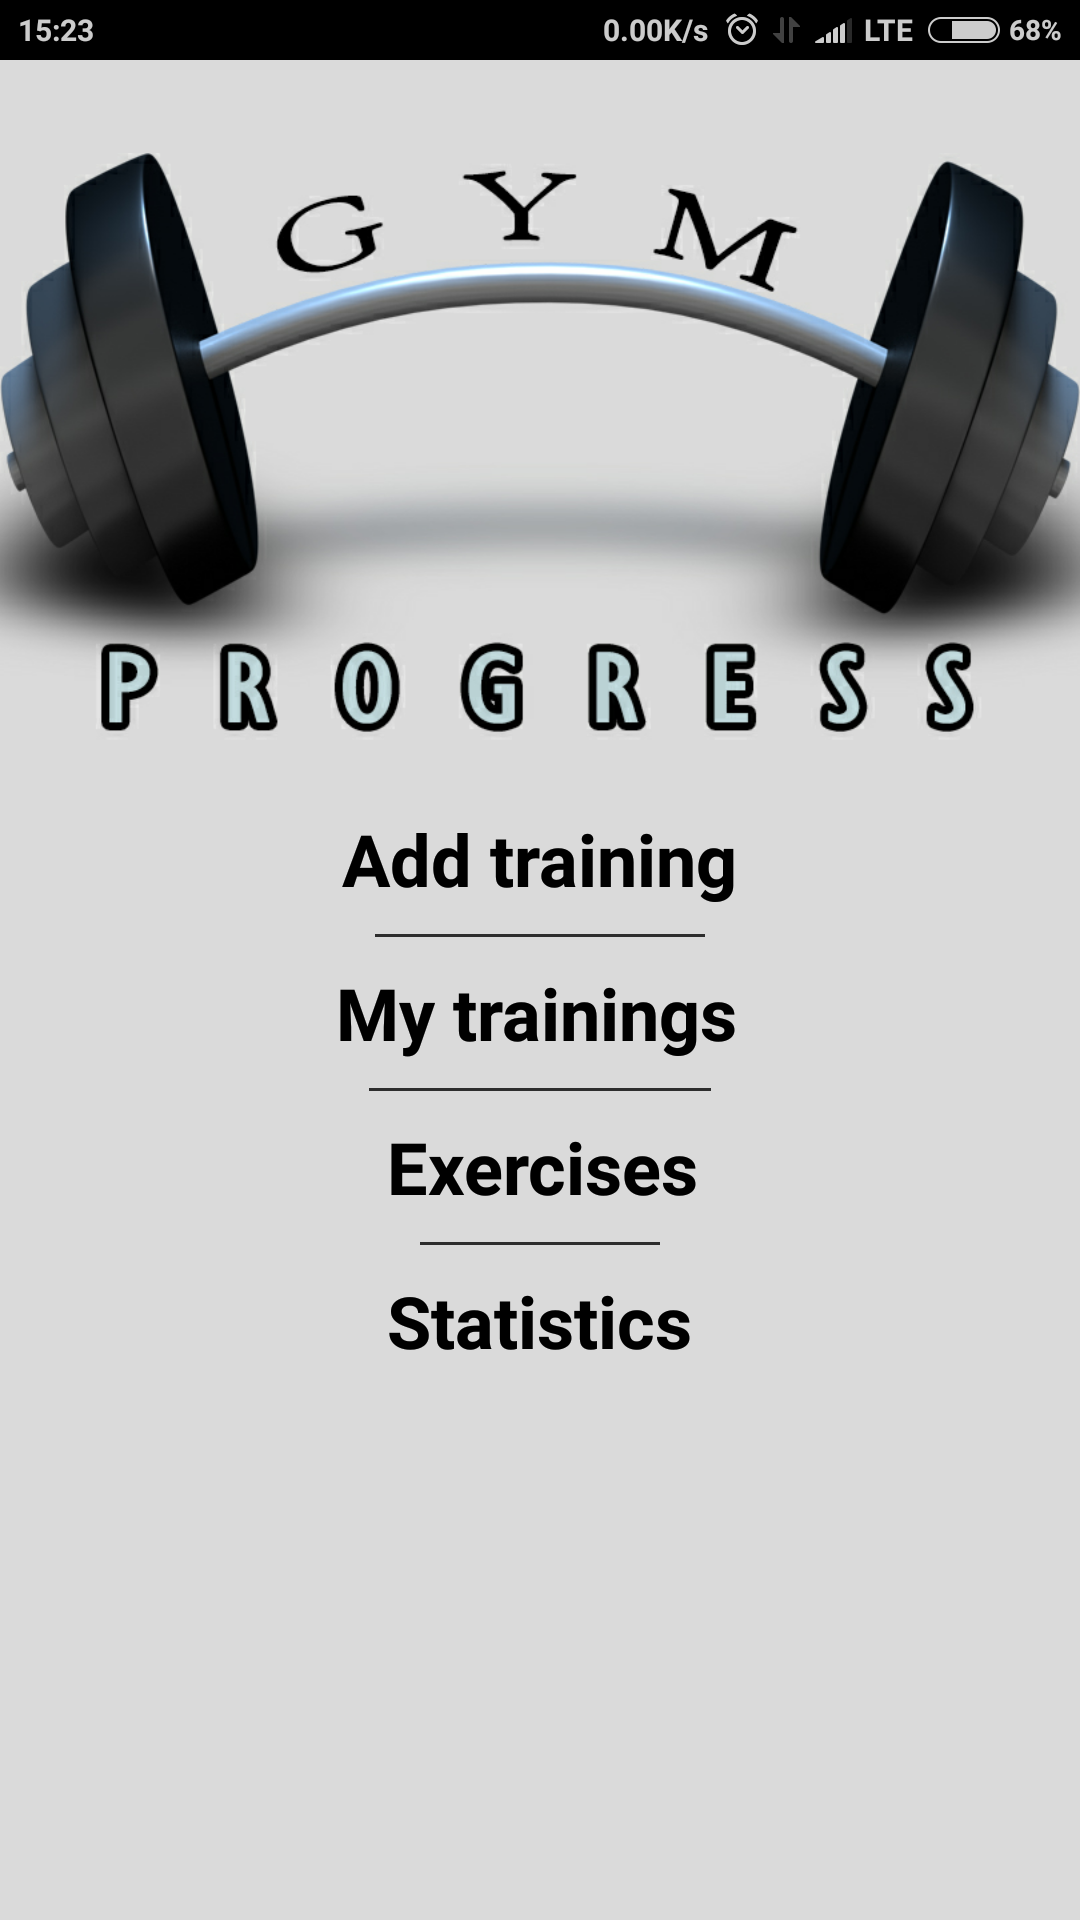
\includegraphics[width=6.75cm,height=12cm]{menu.png}}
\end{center}






\end{document}